\documentclass{standalone}

\ifstandalone
	\usepackage{amsmath}
	\usepackage{pgfplots}
\fi


\begin{document}
	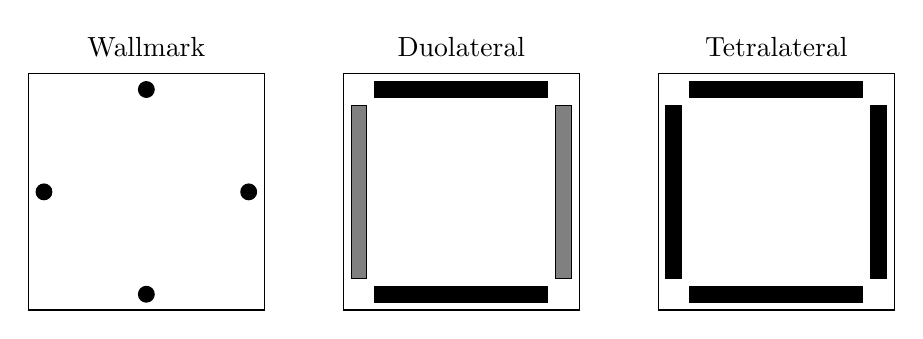
\begin{tikzpicture}
		\filldraw[fill=white] (0, 0) rectangle +(3, 3);
		\filldraw[fill=white] (4, 0) rectangle +(3, 3);
		\filldraw[fill=white] (8, 0) rectangle +(3, 3);
		\filldraw (1.5, 0.2) circle (.1);
		\filldraw (1.5, 2.8) circle (.1);
		\filldraw (0.2, 1.5) circle (.1);
		\filldraw (2.8, 1.5) circle (.1);
		\filldraw (4.4, 0.1) rectangle (6.6, 0.3);
		\filldraw (4.4, 2.7) rectangle (6.6, 2.9);
		\filldraw[fill=black!50] (4.1, 0.4) rectangle (4.3, 2.6);
		\filldraw[fill=black!50] (6.7, 0.4) rectangle (6.9, 2.6);
		\filldraw (8.4, 0.1) rectangle (10.6, 0.3);
		\filldraw (8.4, 2.7) rectangle (10.6, 2.9);
		\filldraw (8.1, 0.4) rectangle (8.3, 2.6);
		\filldraw (10.7, 0.4) rectangle (10.9, 2.6);
		\draw (1.5, 3.1) node[above]{Wallmark};
		\draw (5.5, 3.1) node[above]{Duolateral};
		\draw (9.5, 3.1) node[above]{Tetralateral};
	\end{tikzpicture}
\end{document}
